% !TEX encoding = UTF-8
% !TEX TS-program = pdflatex
% !TEX root = ../tesi.tex

%**************************************************************
\chapter{Strumenti e tecnologie}
\label{cap:strumenti-e-tecnologie}
%**************************************************************

\intro{Analisi e descrizione delle tecnologie utilizzate}\\

%**************************************************************
\section{Strumenti utilizzati}

\subsection{Ambiente di sviluppo}
Durante le 8 settimane di stage, mi è stata assegnata una macchina con sistema operativo Windows 10 64 bit per svolgere il tirocinio universitario. Mi è stato richiesto di utilizzare Virtual Box per poter creare l'ambiente di sviluppo con sistema operativo Debian 10.10 (Buster). \newline{} Virtual Box è un software gratuito e open source per l'esecuzione di macchine virtuali per architettura x86 e 64bit che supporta Windows, GNU/Linux e macOS come sistemi operativi host, ed è in grado di eseguire Windows, GNU/Linux, OS/2 Warp, BSD come ad esempio OpenBSD, FreeBSD e infine Solaris e OpenSolaris come sistemi operativi guest.\newline{}
Nella macchina virtuale in seguito mi è stato consigliato di utilizzare PyCharm come strumento per lo sviluppo del prodotto.\newline{}
PyCharm è un IDE integrato multi-piattaforma per Python; è un software distribuito sotto i termini della Apache License nella sua versione "Community".
\begin{figure}[!h] 
    \centering 
    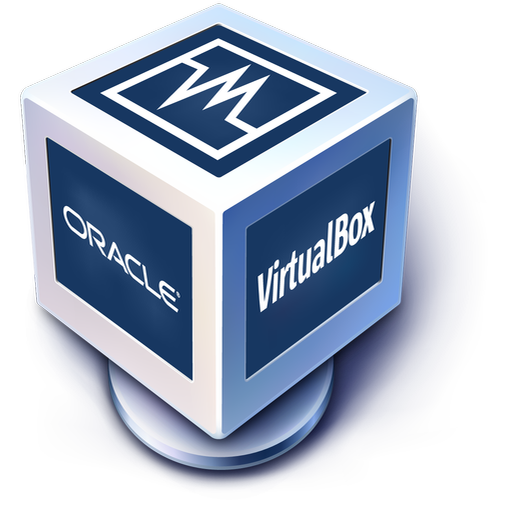
\includegraphics[width=0.1\columnwidth]{logo-virtualbox.png} 
    \caption{Logo Virtualbox}
\end{figure}

\begin{figure}[!h] 
    \centering 
    
\includegraphics[width=0.1\columnwidth]{logo-pycharm.png} 
    \caption{Logo PyCharm}
\end{figure}

\subsection{Strumenti di versionamento}

\subsection{Strumenti aziendali}

\subsection{Altri strumenti}

%**************************************************************
\section{Tecnologie utilizzate}

\subsection{Linguaggi}

\subsection{Framework}
Selenium e robe per test 

%**************************************************************